%!TEX root = ./template-skripsi.tex
%-------------------------------------------------------------------------------
%                            	BAB IV
%               		IMPLEMENTASI DAN PENGUJIAN
%-------------------------------------------------------------------------------

\chapter{HASIL DAN PEMBAHASAN}

\section{Implementasi}

Berikut adalah keterangan \textit{flowchart} tentang apa saja yang telah 
berhasil diimplementasikan. Warna hijau menandakan implementasi telah berhasil 
dibuat, sementara warna merah menandakan implementasi belum sempurna.

\begin{figure}[H]
  \centering{}
	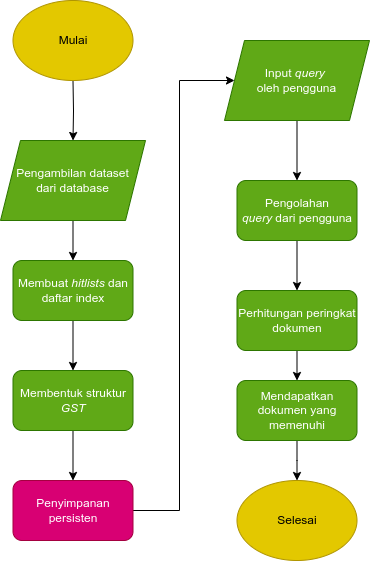
\includegraphics[width=0.7\textwidth]{gambar/flowchart_jadi}
  \caption{\textit{Flowchart} tahapan penelitian yang sudah jadi}
\end{figure}

Untuk penyimpanan persisten saat ini berjalan, tetapi tidak secara
\textit{concurrent} karena keterbatasan kemampuan penulis.

\subsection{Pengolahan \textit{Dataset}}

Sebelum menjalankan modul \textit{indexer}, dataset perlu dikumpulkan terlebih 
dahulu. Proses pengumpulan dataset dilakukan dengan menggunakan modul
\textit{crawler} dari hasil penelitian sebelumnya. Titik pengumpulan dataset 
adalah situs \textit{Forum News Network} (\textit{fnn.co.id}), dengan durasi
\textit{crawling} selama 48 jam. Modul \textit{crawler} dijalankan pada hari
Jum'at, 23 Juni 2023 dan selesai pada hari Minggu, 25 Juni 2023.

Pada database, terdapat dua tabel yang akan digunakan dalam modul
\textit{indexer}. Pertama adalah tabel \textit{page\_paragraph} yang berisi 
seluruh teks dalam \textit{tag} paragraf pada halaman web. Data dari tabel ini 
akan digunakan untuk membentuk struktur index yang akan digunakan dalam proses 
pencarian data. Yang kedua adalah tabel \textit{page\_information} yang berisi
informasi tentang judul dan \textit{URL} dari halaman web. Data dari tabel ini 
akan digunakan untuk mendapatkan detail dari halaman setelah proses kalkulasi 
skor tiap dokumen.

\begin{figure}[H]
  \centering{}
	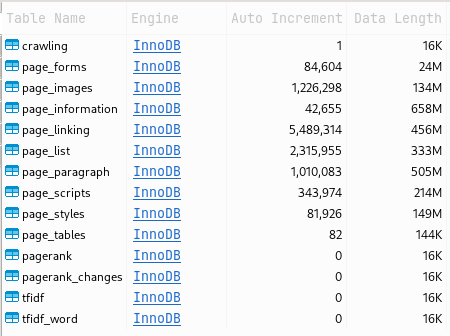
\includegraphics[width=0.7\textwidth]{gambar/implementasi_statistik_dataset}
  \caption{Statistik dataset hasil \textit{crawling}}
\end{figure}

\begin{figure}[H]
  \centering{}
	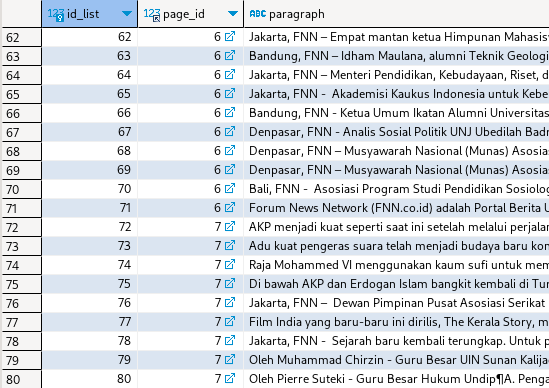
\includegraphics[width=0.85\textwidth]{gambar/implementasi_pageparagraph}
  \caption{Informasi pada tabel \textit{page\_paragraph}}
\end{figure}

\subsection{Pembentukan \textit{Inverted Index}}

Fungsi \textit{getRepoDump} mengambil dataset dari database dengan menggunakan 
objek \textit{Database} yang sudah diinisiasi sebelumnya. Kemudian didapatkan
sebuah \textit{list} berisi pasangan \textit{id} dari dokumen dan paragraf yang
ditemukan pada dokumen tersebut.

\begin{figure}[H]
  \centering{}
	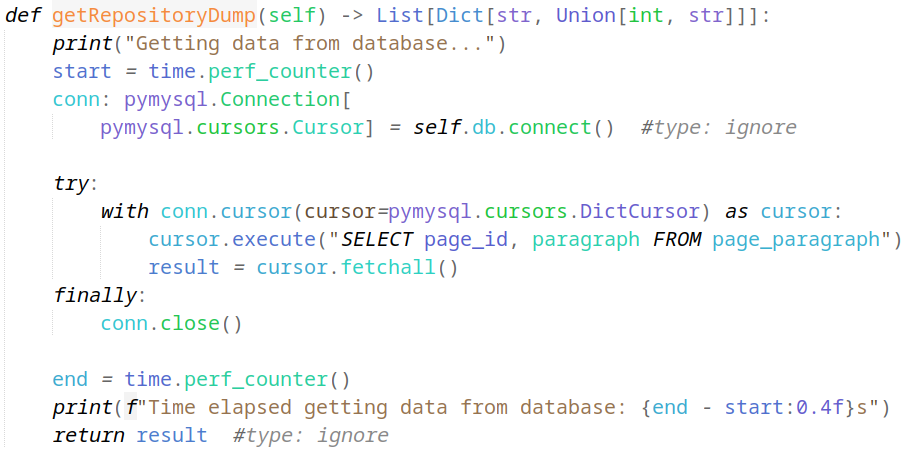
\includegraphics[width=0.85\textwidth]{gambar/implementasi_getrepodump}
  \caption{Pengambilan dataset dari database}
\end{figure}

Setelah dataset didapatkan, fungsi \textit{generateIndex} akan membuat struktur 
index berdasarkan data tersebut. Untuk setiap pasangan pada dataset, paragraf 
akan dikumpulkan berdasarkan \textit{id} dari dokumen. Setelah pemetaan antara 
dokumen dan paragraf selesai dibuat, maka untuk setiap dokumen daftar paragraf 
akan diolah oleh fungsi \textit{generateHitlists}.

\begin{figure}[H]
  \centering{}
	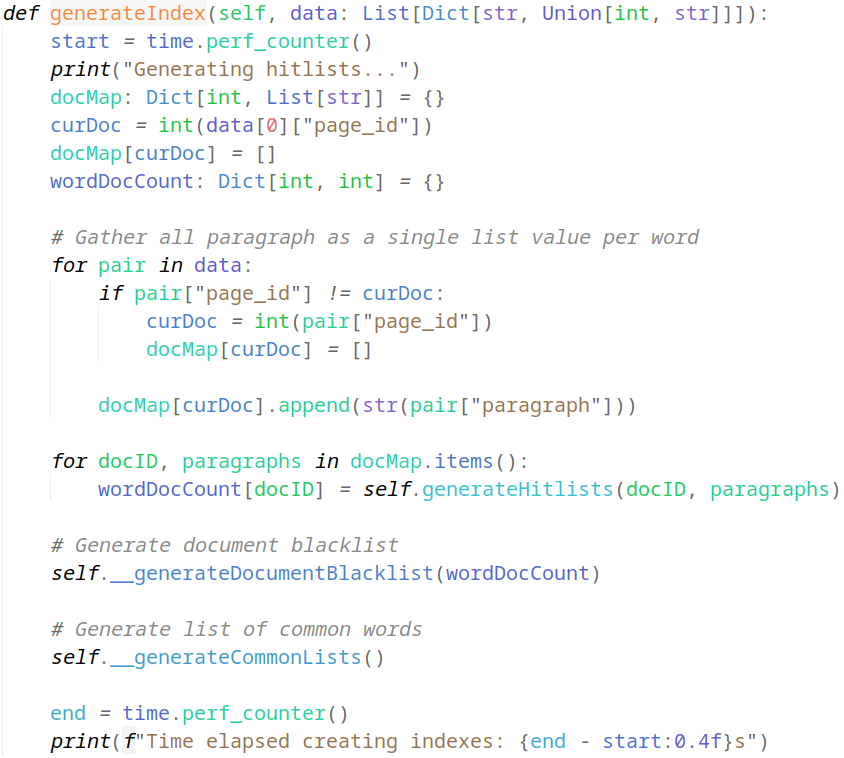
\includegraphics[width=0.85\textwidth]{gambar/implementasi_generateindex}
  \caption{Pembuatan struktur index dari dataset}
\end{figure}

Pada fungsi \textit{generateHitlists}, setiap paragraf akan dibersihkan terlebih 
dahulu sehingga hanya tersisa karakter alfanumerik yang dipisahkan oleh spasi.
Paragraf yang sudah dibersikan kemudian akan dibagi berdasarkan spasi menjadi 
sebuah daftar kata. Kemudian, untuk setiap kata akan disimpan informasi tentang 
\textit{id} dari dokumen saat ini, posisi kata pada dokumen, dan apakah kata 
tersebut termasuk kapital (singkatan dari sebuah istilah).

\begin{figure}[H]
  \centering{}
	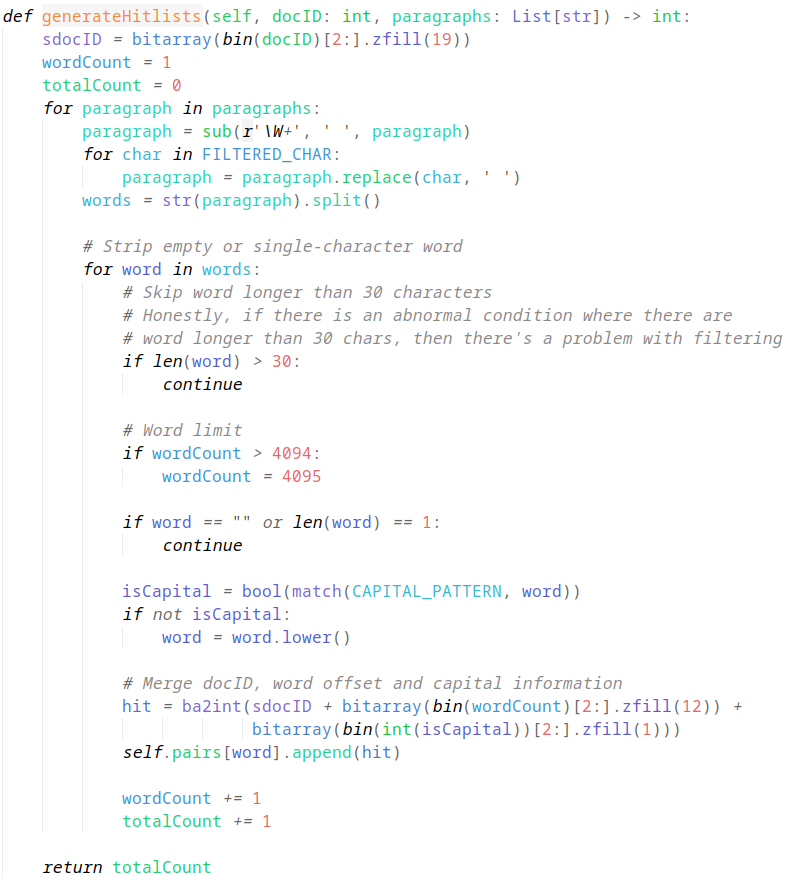
\includegraphics[width=0.85\textwidth]{gambar/implementasi_generatehitlists}
  \caption{Pengolahan paragraf menjadi \textit{hitlist}}
\end{figure}

Fungsi \textit{storeIndex} digunakan untuk menyimpan struktur index pada sebuah
file persisten dengan nama \textit{telusuri\_store.pkl}. File ini nantinya dapat 
langsung digunakan kembali ketika modul tidak menggunakan konfigurasi
\textit{reindex}.

\begin{figure}[H]
  \centering{}
	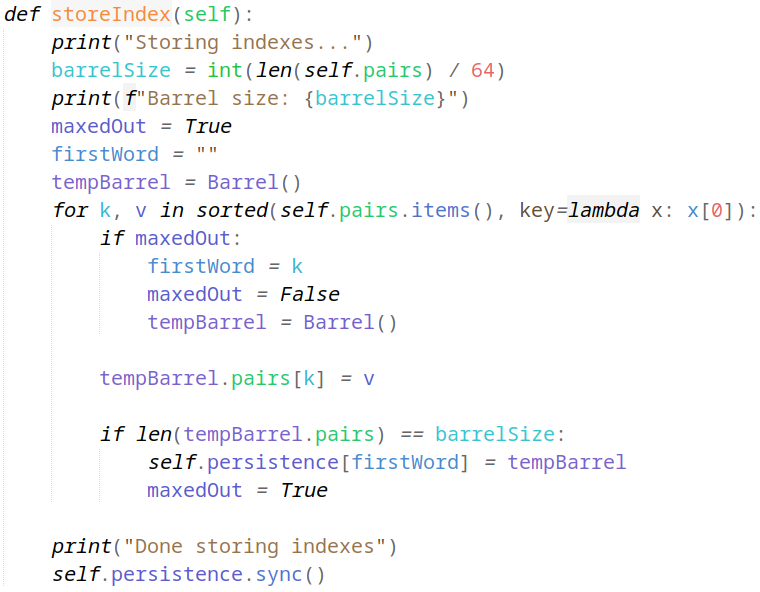
\includegraphics[width=0.85\textwidth]{gambar/implementasi_storeindex}
  \caption{Penyimpanan struktur index ke file persisten}
\end{figure}

\subsection{Pengolahan \textit{User Query}}

Setelah menerima input \textit{query} dari pengguna, teks akan diolah pada 
fungsi \textit{getInputPairs}. Fungsi tersebut akan memecah teks input dari 
pengguna berdasarkan spasi, menjadi sebuah daftar kata yang berurutan. Untuk 
setiap kata pada teks input, akan diolah informasi relatif terhadap teks input.
Informasi tersebut adalah posisi kata pada teks input, apakah kata tersebut 
masuk dalam kategori kata umum dan apakah kata tersebut adalah kata kapital.
Seluruh informasi disimpan dalam sebuah objek \textit{UserQuery}, yang nantinya 
akan menyimpan seluruh informasi yang telah diolah berdasarkan input pengguna.

\begin{figure}[H]
  \centering{}
	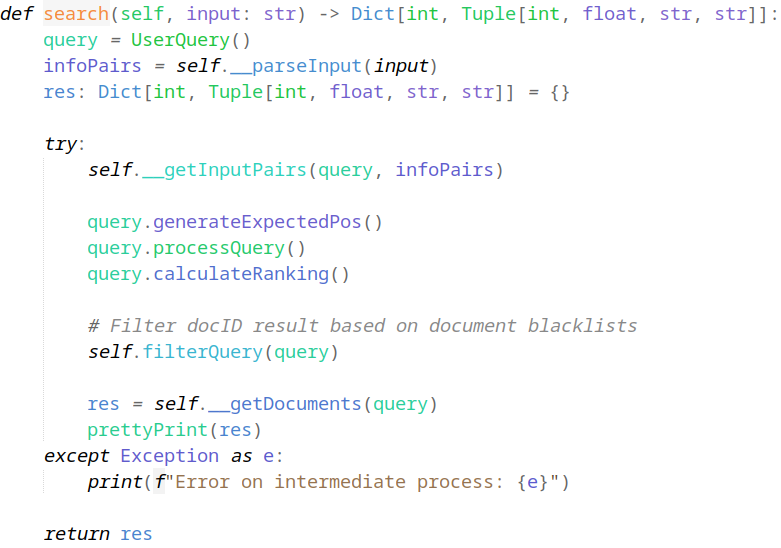
\includegraphics[width=\textwidth]{gambar/implementasi_search}
  \caption{Fungsi pencarian utama}
\end{figure}

\begin{figure}[H]
  \centering{}
	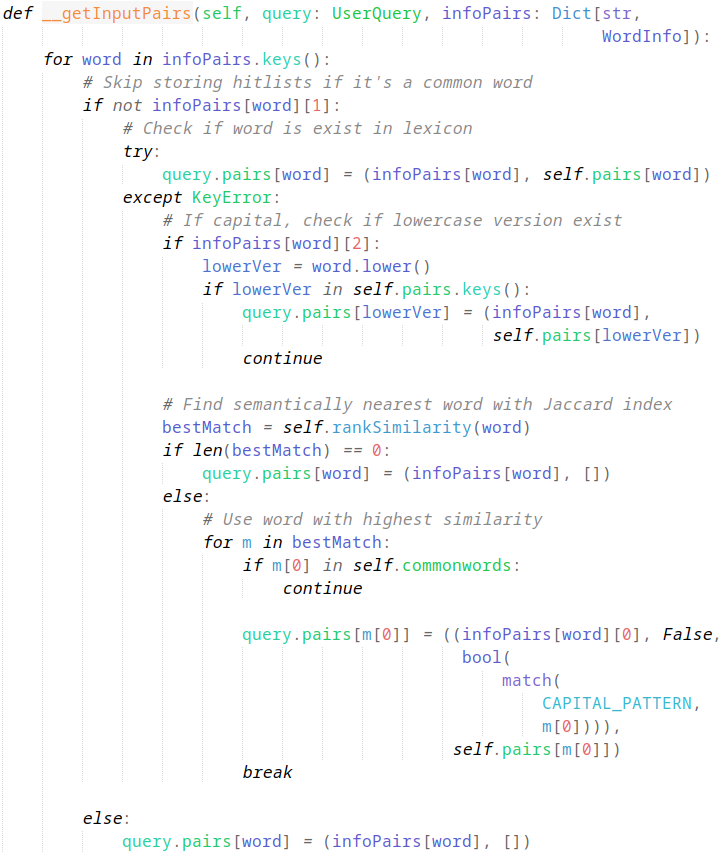
\includegraphics[width=\textwidth]{gambar/implementasi_getinputpairs}
  \caption{Pengolahan teks input dari pengguna}
\end{figure}

Dalam proses pengolahan teks input, untuk setiap kata yang bersifat umum maka 
\textit{hitlist} tidak akan diambil untuk digabungkan karena alasan efisiensi.
Selain itu, untuk kata yang bersifat kapital, apabila kata tersebut tidak ada 
pada daftar kosakata, maka akan dicoba untuk didapatkan varian non-kapitalnya 
terlebih dahulu. Seluruh kata yang sudah didapatkan \textit{hitlist}-nya, 
posisi relatifnya akan dimasukkan ke dalam variabel \textit{expectedPos} untuk 
dibandingkan ketika proses pemeringkatan. Proses ini dilakukan pada fungsi 
\textit{generateExpectedPos}.

\begin{figure}[H]
  \centering{}
	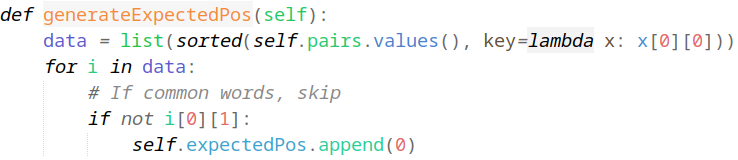
\includegraphics[width=\textwidth]{gambar/implementasi_generateexpectedpos}
  \caption{Fungsi untuk menyimpan posisi yang sesuai dengan teks input 
  berdasarkan urutan}
\end{figure}

Setelah \textit{hitlist} didapatkan pada masing-masing kata, seluruh data akan
digabungkan menjadi satu \textit{hitlist} lengkap, dan kemudian diurutkan dari 
nilai terkecil.

\subsection{Proses Penggabungan \textit{Hitlist} dan Pemeringkatan Hasil}

Pada fungsi \textit{calculateRanking}, akan dilakukan iterasi pada seluruh
\textit{hitlist} untuk menghitung nilai per dokumen. Untuk setiap iterasi,
setiap posisi akan disimpan dalam variabel \textit{curIter}, dan akan dicek 
apakah isi dari variabel tersebut telah sesuai dengan \textit{expectedPos}.
Apabila iterasi telah pindah ke dokumen lain sebelum seluruh kata terkumpul, 
maka dokumen sebelumnya akan masuk dalam golongan \textit{substring match}.
Selain jenis \textit{match}, jumlah kemunculan \textit{match} tersebut juga akan 
disimpan, dan dihitung ketika terjadi perpindahan dokumen pada iterasi.

\begin{figure}[H]
  \centering{}
	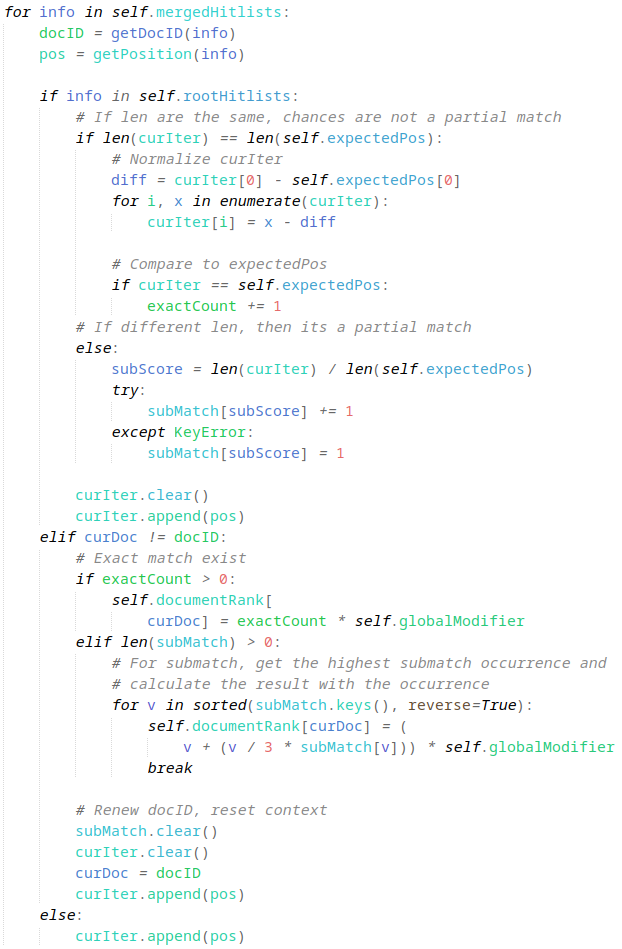
\includegraphics[width=\textwidth]{gambar/implementasi_calculaterank}
  \caption{Proses kalkulasi peringkat}
\end{figure}

Setelah proses pemeringkatan selesai, dokumen akan disaring terlebih dahulu 
berdasarkan variabel \textit{documentBlacklist} melalui fungsi
\textit{filterQuery}. Hasil yang telah disaring akan digunakan untuk mendapatkan
data halaman web dari database. Melalui fungsi \textit{getDocuments}, akan
diambil seluruh data yang mengandung nilai dari seluruh \textit{id} dokumen.
Kemudian, data akan dicetak berdasarkan peringkat dokumen tertinggi.

\begin{figure}[H]
  \centering{}
	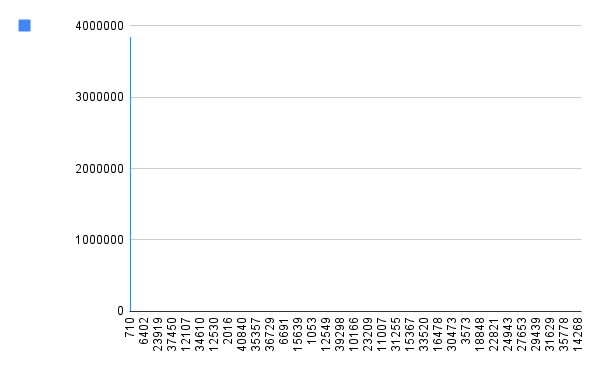
\includegraphics[width=0.92\textwidth]{gambar/word_count}
  \caption{Grafik jumlah kata dalam dokumen}
\end{figure}

\begin{figure}[H]
  \centering{}
	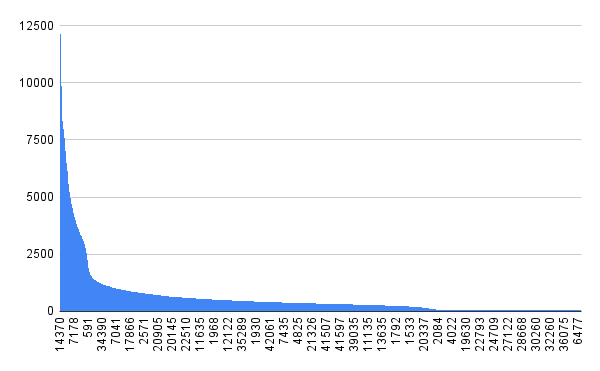
\includegraphics[width=0.7\textwidth]{gambar/word_count2}
  \caption{Grafik jumlah kata dalam dokumen setelah menyingkirkan 20 entri 
  tertinggi}
\end{figure}

\begin{figure}[H]
  \centering{}
	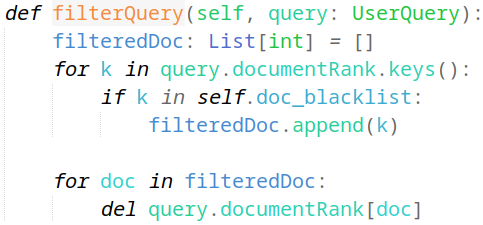
\includegraphics[width=0.85\textwidth]{gambar/implementasi_filterquery}
  \caption{Penyaringan terhadap dokumen yang telah di-\textit{blacklist}}
\end{figure}

\begin{figure}[H]
  \centering{}
	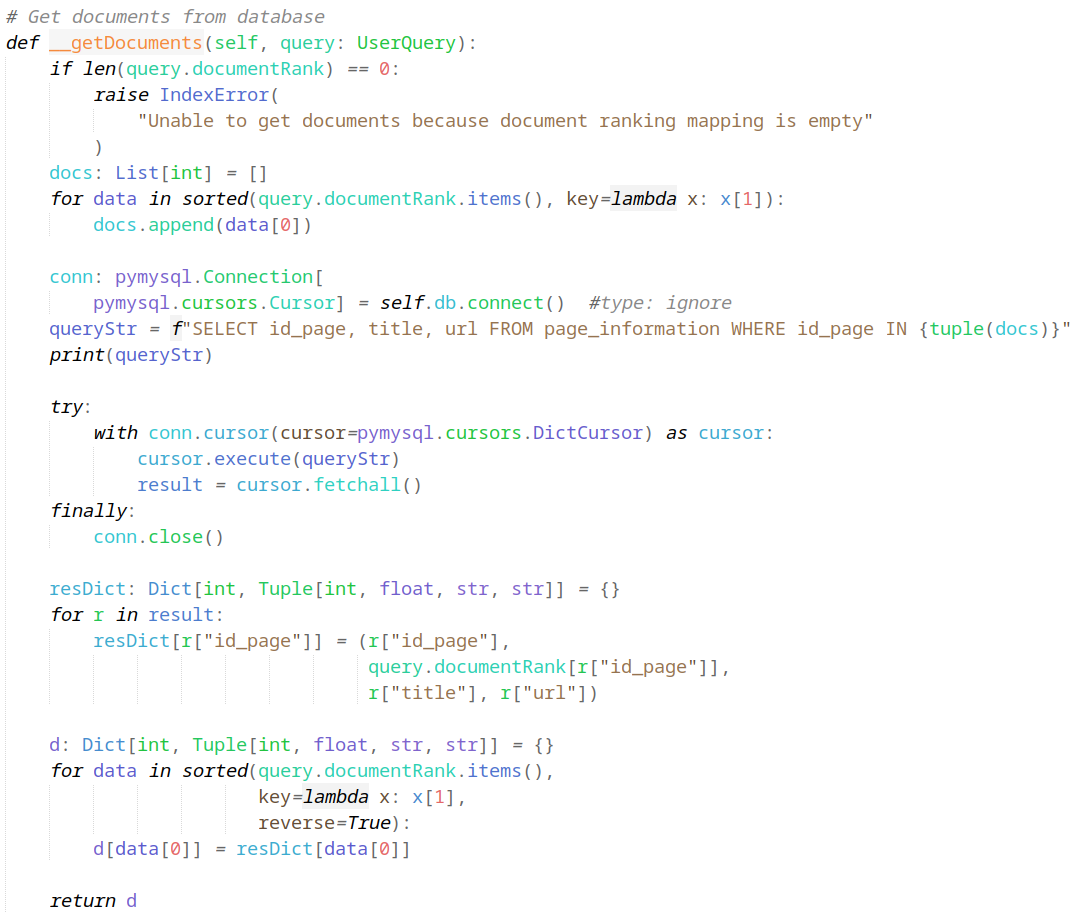
\includegraphics[width=\textwidth]{gambar/implementasi_getdocuments}
  \caption{Pengambilan dokumen dari database dan pemetaan informasi dokumen 
  berdasarkan skor}
\end{figure}

\subsection{Integrasi dengan \textit{Generalized Suffix Tree (GST)}}

Implementasi \textit{GST} yang dipilih adalah implementasi dari hasil penelitian
sebelumnya (\cite{zaidan2023gst}). Tetapi karena kondisi kode yang tidak bisa
langsung digunakan, diperlukan beberapa perbaikan pada kode. Bagian kode yang
perlu diperbaiki adalah penggunaan iterasi yang lebih tepat dan beberapa
penambahan operasi kondisional untuk menangani kesalahan pada data.

Perubahan pertama adalah pada kondisi yang digunakan untuk iterasi ketika 
mengambil informasi dari database. Ditambahkan operasi kondisional untuk 
mengecek apakah kolom \textit{title} tidak bernilai \textit{None} dan memiliki 
panjang lebih dari $0$.

\begin{figure}[H]
  \centering{}
	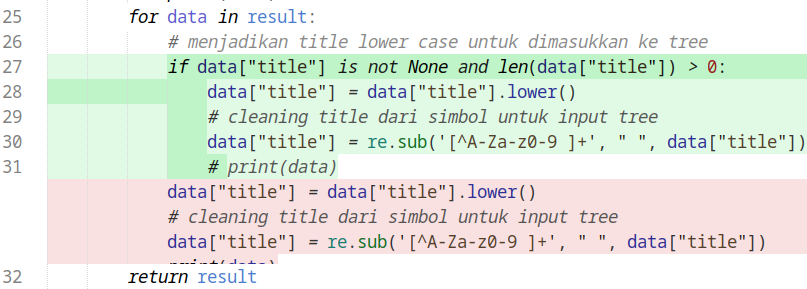
\includegraphics[width=0.7\textwidth]{gambar/implementasi_gstchange2}
  \caption{Perubahan pada iterasi ketika mengambil data dari database}
\end{figure}

Perubahan kedua adalah pada kondisi yang digunakan untuk interasi ketika membuat 
struktur \textit{tree}. Ditambahkan operasi kondisional untuk memastikan bahwa 
nilai dari \textit{title} tidak kosong.

\begin{figure}[H]
  \centering{}
	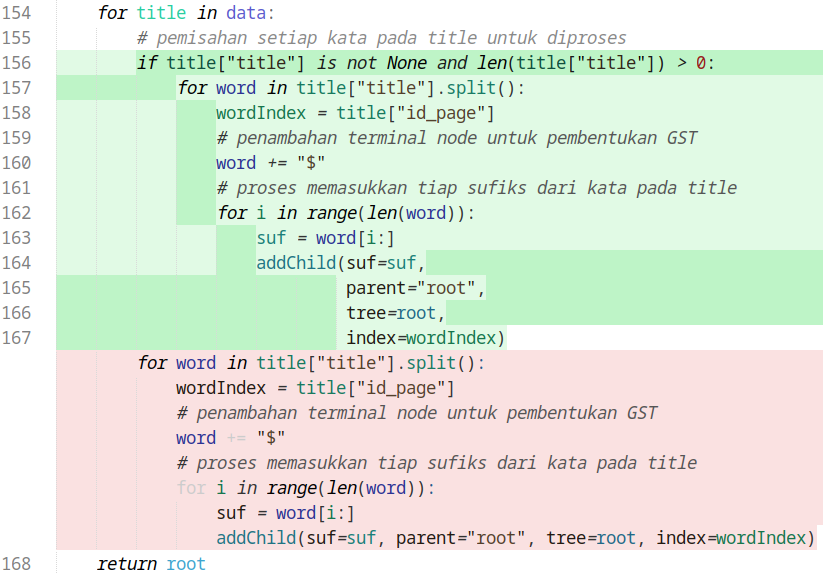
\includegraphics[width=0.7\textwidth]{gambar/implementasi_gstchange3}
  \caption{Perubahan pada iterasi ketika membentuk struktur \textit{tree}}
\end{figure}

Setelah implementasi diperbaiki dan dikonfirmasi dapat berjalan melalui 
pengujian terpisah, dilakukan \textit{refactoring} pada kode untuk memudahkan 
integrasi. \textit{Class GST} dibuat, dan ditambahkan beberapa fungsi untuk 
memudahkan integrasi. Modul \textit{indexer} hanya perlu melakukan impor modul 
untuk dapat menggunakannya.

\begin{figure}[H]
  \centering{}
	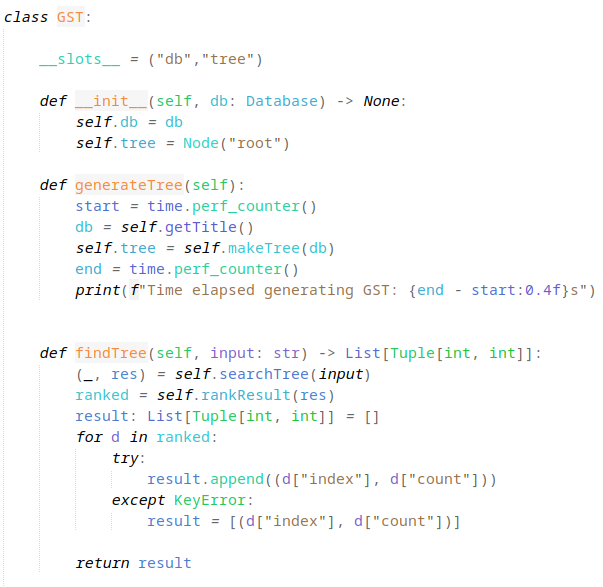
\includegraphics[width=0.7\textwidth]{gambar/implementasi_gst}
  \caption{Implementasi \textit{class GST} untuk memudahkan integrasi}
\end{figure}

Selain itu, agar lebih mudah dalam proses pengujian, implementasi diberikan 
sebuah \textit{guard} kondisional agar dapat dinyalakan / dimatikan dengan 
menggunakan \textit{environment variable}.

Untuk mengakomodasi implementasi \textit{GST}, terdapat beberapa penambahan 
kode. Yang pertama adalah pemetaan antara dokumen dengan \textit{hitlists}. Untuk 
itu dibuat variabel \textit{documentPairs}. Variabel ini akan menambahkan
\textit{hit} dalam fungsi \textit{generateIndex}, tetapi akan ditambahkan per 
dokumen.

\begin{figure}[H]
  \centering{}
	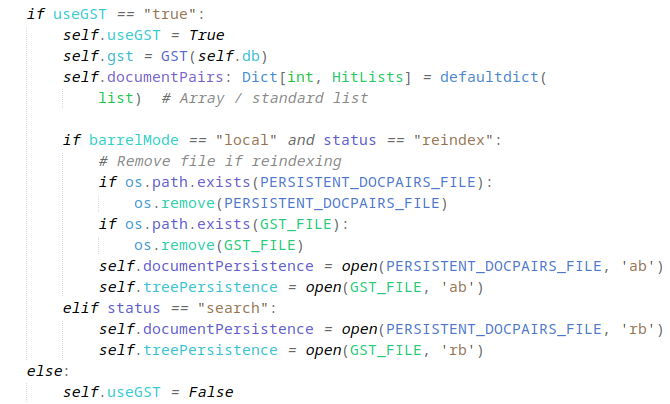
\includegraphics[width=0.7\textwidth]{gambar/implementasi_gst_init}
  \caption{Penambahan inisiasi variabel untuk akomodasi penggunaan \textit{GST}}
\end{figure}

Selanjutnya, pada proses pengolahan \textit{query}, dibuat sebuah fungsi baru 
yaitu \textit{calculateRankingGST}. Karena bentuk input yang berupa daftar
\textit{hitlists} berdasarkan pemetaan dokumen, maka proses perhitungan 
peringkat agak berubah. Proses perhitungan menghindari iterasi secara menyeluruh 
dari \textit{hitlist} dengan cara mengambil irisan dari \textit{hit} yang sesuai 
dengan kata dan dokumen. Dari hasil irisan yang sesuai, barulah perhitungan 
peringkat dimulai.

\begin{figure}[H]
  \centering{}
	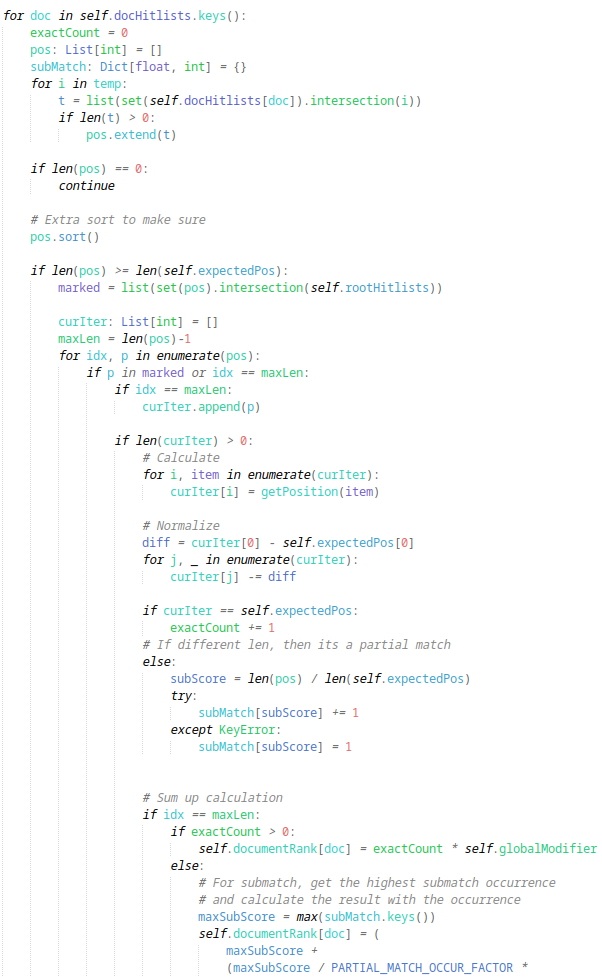
\includegraphics[width=0.7\textwidth]{gambar/implementasi_gst_calculateranking}
  \caption{Perubahan implementasi perhitungan peringkat untuk integrasi
  \textit{GST}}
\end{figure}

Yang terakhir adalah penambahan fungsi untuk mengambil \textit{hitlist} dari 
pemetaan dokumen. Fungsi \textit{getDocumentPairs} dimulai dengan melakukan 
input kata ke modul \textit{GST}. Untuk setiap kata, modul \textit{GST} akan 
mengembalikan daftar dokumen yang memiliki kata tersebut beserta jumlah-nya. 
Dokumen kemudian akan diurutkan berdasarkan jumlah kata, dan untuk setiap 
dokumen akan diambil \textit{hitlist} yang memenuhi.

\begin{figure}[H]
  \centering{}
	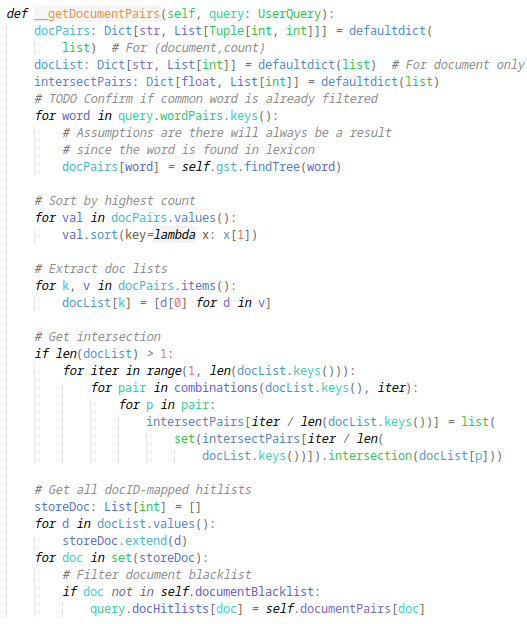
\includegraphics[width=0.7\textwidth]{gambar/implementasi_gst_getdocumentpairs}
  \caption{Fungsi untuk mengambil dokumen berdasarkan hasil dari \textit{GST}}
\end{figure}

\subsection{Modifikasi kode \textit{TF-IDF}}

Metode \textit{TF-IDF} digunakan sebagai patokan untuk memverifikasi kesesuaian 
kata pada hasil pencarian. Kode yang berdasarkan implementasi pemeringkatan 
dokumen pada penelitian sebelumnya. Kode tersebut tidak bisa dijalankan secara 
langsung karena penggunaan \textit{dataset} yang besar membuat proses skoring 
kata dalam dokumen terlalu lama.

Modifikasi yang dilakukan adalah dengan membagi operasi menjadi beberapa bagian, 
dan menyimpan hasil dari setiap operasi kedalam file persisten untuk menghindari 
melakukan proses ulang data.

Operasi pertama yang dilakukan adalah melakukan penyaringan terhadap dataset
yang ada. Agar metode \textit{TF-IDF} dapat bekerja dengan baik, maka dataset
perlu dibersihkan dari kata sambung, atau disisakan kata dasar saja. Metode yang
dipilih adalah penyaringan untuk menyisakan kata dasar saja. Untuk mengetahui 
apakah sebuah kata termasuk kata dasar, diperlukan sebuah daftar yang berisi 
kata dasar untuk digunakan sebagai patokan. Daftar kata yang digunakan diambil 
dari proyek \textit{Sastrawi} (\cite{sastrawi}).

\begin{figure}[H]
  \centering{}
	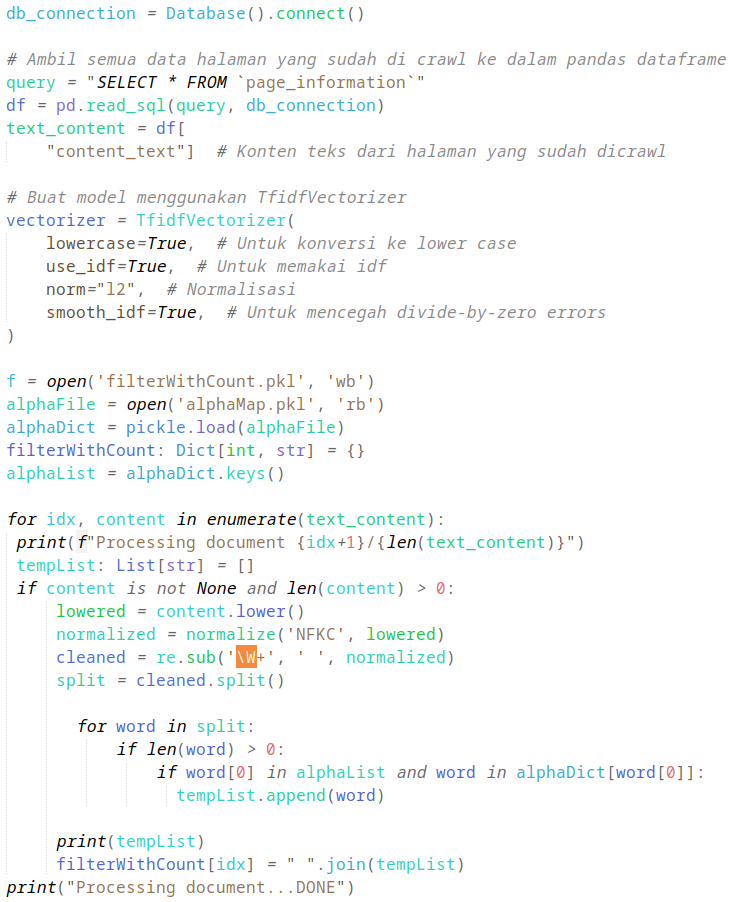
\includegraphics[width=\textwidth]{gambar/implementasi_filterkatadasar.png}
  \caption{Operasi filter pada seluruh dataset dari \textit{table\_information} 
  untuk menyisakan seluruh kemunculan kata dasar pada tiap dokumen}
\end{figure}

Pada percobaan awal, proses filter secara langsung masih memakan waktu yang 
cukup signifikan karena daftar kata dasar yang cukup besar (29932 kata). Oleh 
karena itu, dibuat pemetaan antara huruf pertama dari kata dasar ke seluruh kata 
yang memiliki huruf pertama yang sama.

Setelah terbentuk \textit{dataset} yang telah di filter, seluruh data tersebut 
dimasukkan ke dalam database. Untuk menghindari hal yang tidak diinginkan, 
dibuat salinan tabel \textit{page\_information} ke tabel baru
\textit{page\_information\_filtered} yang nantinya akan menjadi sumber data 
pengganti. Kolom \textit{content\_text} kemudian diperbarui dengan data yang 
sudah di filter.

\begin{figure}[H]
  \centering{}
	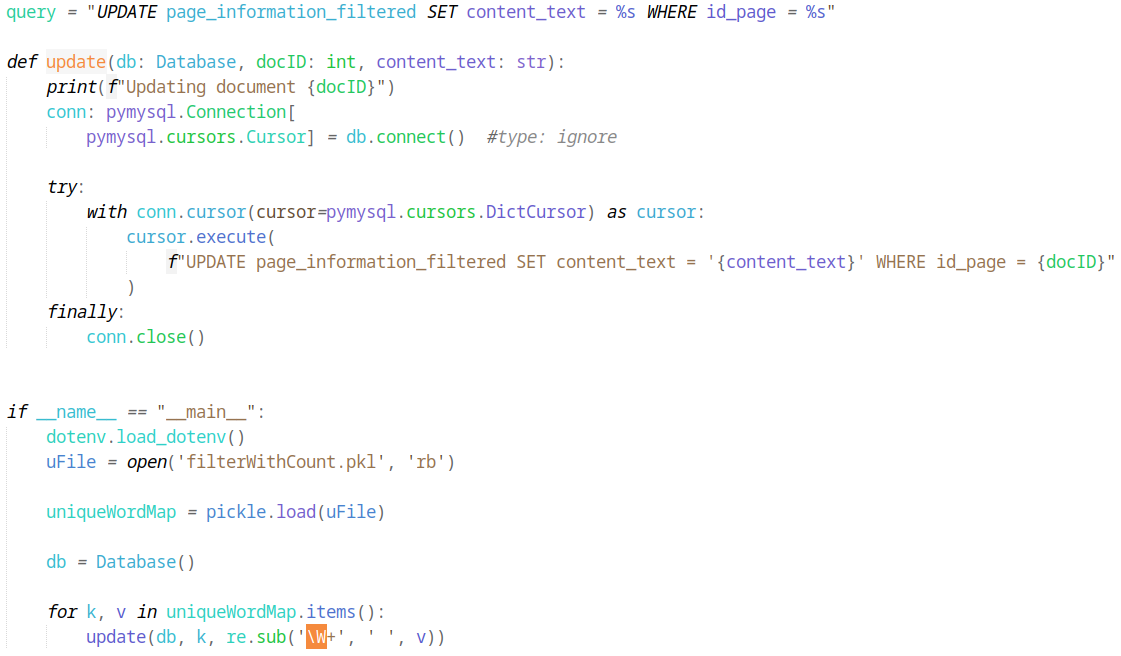
\includegraphics[width=\textwidth]{gambar/implementasi_pageinfo_filtered.png}
  \caption{Pengisian tabel \textit{page\_information\_filtered} dengan data yang 
  sudah di filter dengan daftar kata dasar}
\end{figure}

Operasi selanjutnya adalah pembuatan peringkat kata per dokumen. Pada 
implementasi sebelumnya, setiap kata yang telah mendapatkan skor akan segera di 
masukkan nilainya ke database. Karena proses ini diidentifikasi sebagai proses 
yang paling memperlambat pembuatan skoring kata, maka operasi database dipisah 
dan dilakukan setelah seluruh skor kata per dokumen terbentuk.

\begin{figure}[H]
  \centering{}
	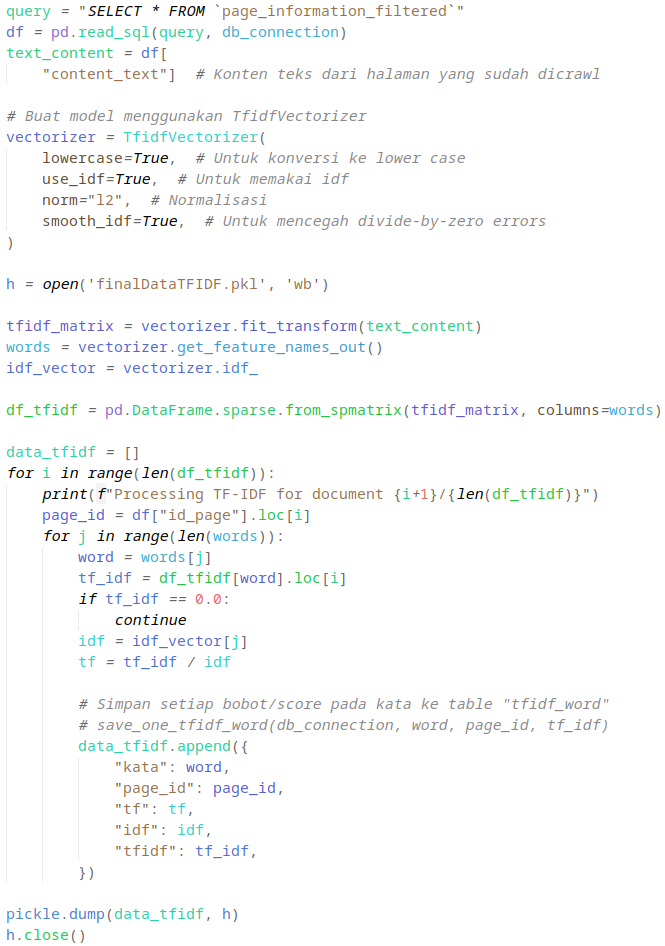
\includegraphics[width=\textwidth]{gambar/implementasi_generate_tfidf.png}
  \caption{Proses skoring kata dari data yang sudah di filter}
\end{figure}

\begin{figure}[H]
  \centering{}
	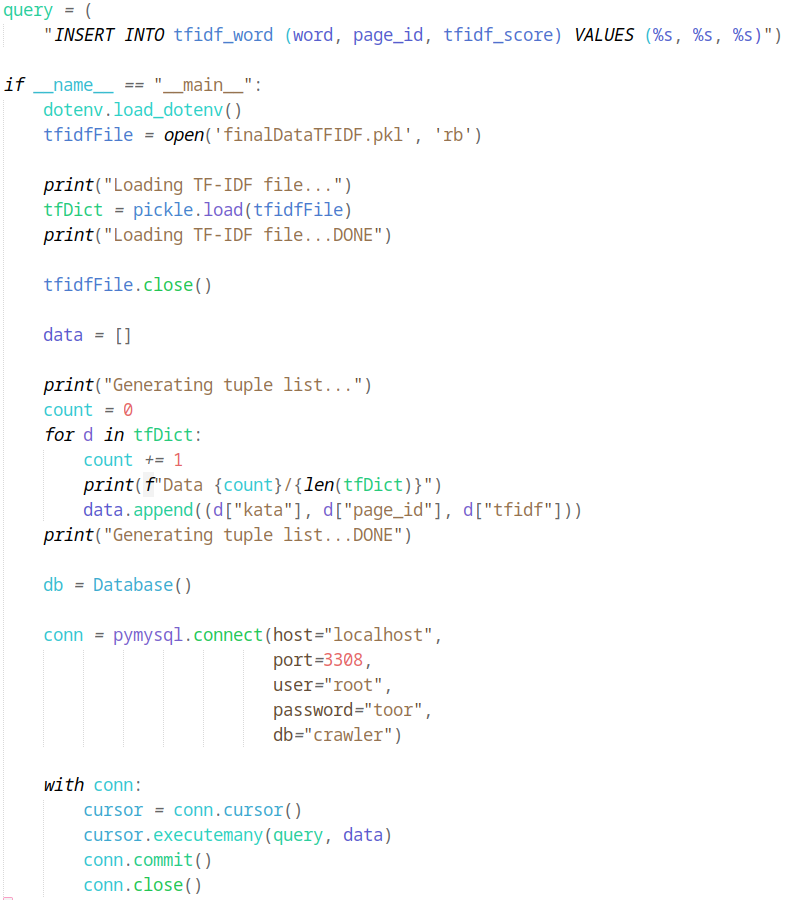
\includegraphics[width=\textwidth]{gambar/implementasi_insert_tfidfword.png}
  \caption{Pengisian tabel \textit{tfidf\_word} dari file persisten}
\end{figure}

\begin{figure}[H]
  \centering{}
	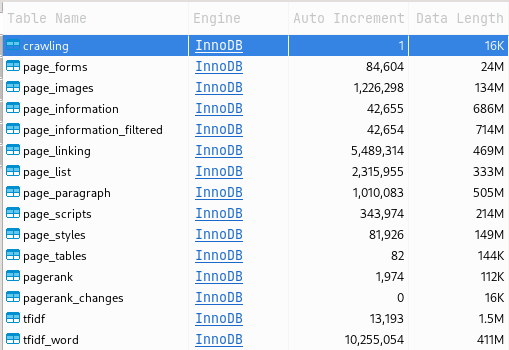
\includegraphics[width=0.7\textwidth]{gambar/implementasi_statistik_dataset_filtered}
  \caption{Statistik dataset setelah proses \textit{filtering}}
\end{figure}

\subsection{Struktur Direktori Kode}

Struktur penulisan kode yang digunakan mengikuti struktur yang telah ada pada 
penelitian sebelumnya. Pada direktori \textit{src}, dibuat folder baru dengan 
nama \textit{indexing} sebagai penanda modul baru. Kemudian di dalamnya terdapat 
file \textit{inverted\_index.py} sebagai tempat implementasi utama.

Untuk menjalankan modul \textit{indexer}, pada direktori utama dibuat file
\textit{run\_index.py} yang memanggil objek dari modul \textit{inverted\_index}.

\section{Pengujian}

\subsection{Statistik Pengujian}

Pengujian dimulai dengan merekam waktu yang terpakai dalam proses pembuatan
struktur index berdasarkan data dari database.

\begin{table}[H]
\begin{center}
  \caption{\label{tabel:durasi_reindex} Durasi proses \textit{reindexing}}
\begin{tabular}{|c|c|c|c|} 
 \hline
  \textit{Mode} & Percobaan Ke-1 & Percobaan Ke-2 & Percobaan Ke-3 \\ 
 \hline
  Pengambilan \textit{dataset} & 7.6138s & 7.5740s & 7.5910s \\
  Inverted Index & 204.2576s & 209.5963s & 204.3641s \\ 
  Inverted Index + GST & 526.0686s & 527.3835s & 535.1130s \\
 \hline
\end{tabular}
\end{center}
\end{table}

Karena terdapat peningkatan signifikan dalam pembuatan index dengan integrasi 
\textit{GST}, maka direkam waktu pembuatan untuk struktur \textit{GST} sendiri.

\begin{table}[H]
\begin{center}
  \caption{\label{tabel:durasi_gst} Durasi pembuatan struktur \textit{GST}}
\begin{tabular}{|c|c|} 
 \hline
  Percobaan & Durasi \\ 
 \hline
  1 & 302.1005s \\ 
  2 & 308.6661s \\
  3 & 319.0878s \\
 \hline
\end{tabular}
\end{center}
\end{table}

Selanjutnya adalah merekam waktu yang digunakan untuk menyimpan struktur yang 
telah dibuat ke dalam file persisten dengan modul \textit{pickle}.

\begin{table}[H]
\begin{center}
  \caption{\label{tabel:durasi_store} Durasi proses penyimpanan struktur data 
  ke file persisten}
\begin{tabular}{|c|c|c|c|} 
 \hline
  \textit{Mode} & Percobaan Ke-1 & Percobaan Ke-2 & Percobaan Ke-3 \\ 
 \hline
  Inverted Index & 6.3289s & 6.1939s & 6.2439s \\ 
  Inverted Index + GST & 6.2494s & 6.2009s & 6.6043s \\
 \hline
\end{tabular}
\end{center}
\end{table}

Setelah itu, direkam proses muat ulang dari file persisten ke struktur data asli
pada memori sebelum digunakan untuk pencarian.

\begin{table}[H]
\begin{center}
  \caption{\label{tabel:durasi_restore} Durasi proses muat ulang struktur data 
  dari file persisten}
\begin{tabular}{|c|c|c|c|} 
 \hline
  Struktur & Percobaan Ke-1 & Percobaan Ke-2 & Percobaan Ke-3 \\ 
 \hline
  Pemetaan Kata -- \textit{Hitlists} & 2.2921s & 2.3181s & 2.2682s \\
  Pemetaan Dokumen -- \textit{Hitlists} & 1.9319s & 1.9767s & 1.9284s \\ 
  GST & 2.1220s & 2.1438s & 2.1274s \\
 \hline
\end{tabular}
\end{center}
\end{table}

Berikut adalah beberapa statistik penggunaan memori dan media penyimpanan yang
dikumpulkan selama pengujian berlangsung.

\begin{table}[H]
\begin{center}
  \caption{\label{tabel:ukuran_struktur} Ukuran struktur data yang terbentuk}
\begin{tabular}{|c|c|c|} 
 \hline
  Struktur & Ukuran di memori & Ukuran file persisten \\ 
 \hline
  Pemetaan Kata -- \textit{Hitlists} & 2035.57 MB & 264 MB \\ 
  Pemetaan Dokumen -- \textit{Hitlists} & 2026.64 MB & 263 MB \\
  GST & 93.75 MB & 7.3 MB \\
 \hline
\end{tabular}
\end{center}
\end{table}

\subsection{Pengujian Relevansi}

Berikut adalah kata kunci yang digunakan untuk uji relevansi hasil pencarian.
Kata kunci dipilih karena dapat digunakan dengan metode \textit{TF-IDF} sebagai 
patokan. Implementasi \textit{TF-IDF} sendiri sepertinya masih memiliki masalah 
di mana terdapat sekumpulan kata yang tidak menghasilkan output apa pun dengan 
menggunakan \textit{dataset} yang digunakan. Sempat dilakukan pengujian dengan 
menggunakan \textit{dataset} baru yang lebih kecil, dan berhasil. Tetapi tetap 
gagal untuk \textit{dataset} utama.

\begin{center}
\begin{longtable}{|c|c|} 
  \caption{\label{tabel:daftar_query} \textit{Query} yang digunakan untuk uji 
  relevansi}\\
 \hline
  \textit{Query} satu kata & \textit{Query} dua kata \\ 
 \hline
  bupati & ganjar pranowo \\ 
  waskita & tiket coldplay \\
  nuklir &  \\
 \hline
\end{longtable}
\end{center}

% Berikut adalah hasil pencarian dengan kata kunci \textit{bupati}.

\begin{center}
\begin{longtable}{|c|c|} 
  \caption{\label{tabel:hasil_inv_bupati} Hasil pencarian dengan kata kunci
  \textit{bupati} dengan metode \textit{inverted index}}\\

  \hline
  % First page header
  \multicolumn{1}{|c|}{\textbf{Peringkat}} & \multicolumn{1}{|c|}{\textbf{Hasil}}\\ \hline 
  \endfirsthead

  % Next page header
  \multicolumn{2}{c}%
    {{\textbf{\tablename\ \thetable{}:} Hasil pencarian dengan kata kunci
  \textit{bupati} dengan metode \textit{inverted index} }} \\
  \hline
  \multicolumn{1}{|c|}{\textbf{Peringkat}} & \multicolumn{1}{|c|}{\textbf{Hasil}}\\ \hline 
  \endhead

  % Next page indication footer
  \hline \multicolumn{2}{|r|}{{Dilanjutkan pada halaman berikutnya}} \\ \hline
  \endfoot

  % Last footer without next page indication
  \hline \hline
  \endlastfoot

 \hline
  1 & Mochamad Toha \\ 
   & \textit{http://fnn.co.id/author/Mochamad Toha} \\
 \hline
  2 & daerah \\
   & \textit{http://fnn.co.id/category/daerah?page=5} \\
 \hline
  3 & kesehatan \\
   & \textit{http://fnn.co.id/category/kesehatan?page=13} \\
 \hline
  4 & nasional \\
   & \textit{http://fnn.co.id/category/nasional?page=11} \\
 \hline
  5 & daerah \\
   & \textit{http://fnn.co.id/category/daerah?page=11} \\
 \hline
\end{longtable}
\end{center}

\begin{center}
  \begin{longtable}[c]{|p{0.2\textwidth}|p{0.8\textwidth}|} 
  \caption{\label{tabel:hasil_gst_bupati} Hasil pencarian dengan kata kunci
  \textit{bupati} dengan metode \textit{inverted index} dan integrasi dengan
  \textit{GST}} \\

  \hline
  % First page header
    \multicolumn{1}{|p{0.2\textwidth}|}{\textbf{Peringkat}} & \multicolumn{1}{|p{0.8\textwidth}|}{\textbf{Hasil}}\\ \hline 
  \endfirsthead

  % Next page header
    \multicolumn{2}{p{\textwidth}}%
    {{\textbf{\tablename\ \thetable{}:} Hasil pencarian dengan kata kunci
  \textit{bupati} dengan metode \textit{inverted index} dan integrasi dengan
    \textit{GST}}} \\
  \hline
    \multicolumn{1}{|p{0.2\textwidth}|}{\textbf{Peringkat}} & \multicolumn{1}{|p{0.8\textwidth}|}{\textbf{Hasil}}\\ \hline 
  \endhead

  % Next page indication footer
  \hline \multicolumn{2}{|r|}{{Dilanjutkan pada halaman berikutnya}} \\ \hline
  \endfoot

  % Last footer without next page indication
  \hline \hline
  \endlastfoot

 \hline
  1 & Selain Bupati Saiful Ilah, Ada Raja Koruptor yang Sedang diburu KPK! \\ 
   & \textit{http://fnn.co.id/post/selain-bupati-saiful-ilah-ada-raja-koruptor-yang-sedang-diburu-kpk} \\
 \hline
  2 & Ruslan Tawari: Pejabat Bupati Seram Barat Jangan Bikin Resah Rakyat \\
   & \textit{http://fnn.co.id/post/rustlam-tawari-pejabat-bupati-seram-barat-jangan-bikin-resah-rakyat-\#back-to-top} \\
 \hline
  3 & Ruslan Tawari: Pejabat Bupati Seram Barat Jangan Bikin Resah Rakyat \\
   & \textit{http://fnn.co.id/post/rustlam-tawari-pejabat-bupati-seram-barat-jangan-bikin-resah-rakyat-\#1} \\
 \hline
  4 & Ruslan Tawari: Pejabat Bupati Seram Barat Jangan Bikin Resah Rakyat \\
   & \textit{http://fnn.co.id/post/rustlam-tawari-pejabat-bupati-seram-barat-jangan-bikin-resah-rakyat-\#1} \\
 \hline
  5 & Ruslan Tawari: Pejabat Bupati Seram Barat Jangan Bikin Resah Rakyat \\
   & \textit{http://fnn.co.id/post/rustlam-tawari-pejabat-bupati-seram-barat-jangan-bikin-resah-rakyat-\#1} \\
 \hline
\end{longtable}
\end{center}

\begin{center}
  \begin{longtable}[c]{|p{0.2\textwidth}|p{0.8\textwidth}|} 
  \caption{\label{tabel:hasil_tfidf_bupati} Hasil pencarian dengan kata kunci
  \textit{bupati} dengan metode \textit{TF-IDF}} \\

  \hline
  % First page header
    \multicolumn{1}{|p{0.2\textwidth}|}{\textbf{Peringkat}} & \multicolumn{1}{|p{0.8\textwidth}|}{\textbf{Hasil}}\\ \hline 
  \endfirsthead

  % Next page header
  \multicolumn{2}{c}%
    {{\textbf{\tablename\ \thetable{}:} Hasil pencarian dengan kata kunci
    \textit{bupati} dengan metode \textit{TF-IDF}}} \\
  \hline
  \multicolumn{1}{|c|}{\textbf{Peringkat}} & \multicolumn{1}{|c|}{\textbf{Hasil}}\\ \hline 
  \endhead

  % Next page indication footer
  \hline \multicolumn{2}{|r|}{{Dilanjutkan pada halaman berikutnya}} \\ \hline
  \endfoot

  % Last footer without next page indication
  \hline \hline
  \endlastfoot

 \hline
    1 & \textit{http://fnn.co.id/post/jahiliyah-yang-belum-berevolusi} \\ 
 \hline
    2 & \textit{http://fnn.co.id/post/wakil-ketua-dpr-santri-harus-jadi-penopang-kekuatan-ekonomi-baru} \\
 \hline
    3 & \textit{http://fnn.co.id/post/pemprov-sulsel-resmikan-ruas-jalan-perbatasan-sidrap-soppeng} \\
 \hline
    4 & \textit{http://fnn.co.id/category/daerah?page5\#back-to-top} \\
 \hline
    5 & \textit{http://fnn.co.id/category/daerah?page=18\#3} \\
 \hline
\end{longtable}
\end{center}

% Bupati

% Berikut adalah hasil pencarian dengan kata kunci \textit{waskita}.

\begin{center}
\begin{longtable}{|c|c|} 
  \caption{\label{tabel:hasil_inv_waskita} Hasil pencarian dengan kata kunci
  \textit{waskita} dengan metode \textit{inverted index}} \\

  \hline
  % First page header
  \multicolumn{1}{|c|}{\textbf{Peringkat}} & \multicolumn{1}{|c|}{\textbf{Hasil}}\\ \hline 
  \endfirsthead

  % Next page header
  \multicolumn{2}{|c|}%
    {{\textbf{\tablename\ \thetable{}:} \textit{Inverted file index} dari lirik lagu pada tabel
    \ref{tab:lirik}}} \\
  \multicolumn{1}{|c|}{\textbf{Peringkat}} & \multicolumn{1}{|c|}{\textbf{Hasil}}\\ \hline 
  \endhead

  % Next page indication footer
  \hline \multicolumn{2}{r}{{Dilanjutkan pada halaman berikutnya}} \\ \hline
  \endfoot

  % Last footer without next page indication
  \hline \hline
  \endlastfoot
 % \hline
 %  Peringkat & Hasil \\ 
 \hline
  1 & Dimas Huda \\ 
   & \textit{http://fnn.co.id/author/Dimas Huda} \\
 \hline
  2 & infrastruktur \\
   & \textit{http://fnn.co.id/category/infrastruktur} \\
 \hline
  3 & hukum \\
   & \textit{http://fnn.co.id/category/hukum?page=4} \\
 \hline
  4 & Mochamad Toha \\
   & \textit{http://fnn.co.id/author/Mochamad Toha} \\
 \hline
  5 & editorial \\
   & \textit{http://fnn.co.id/category/editorial} \\
 \hline
\end{longtable}
\end{center}

\begin{table}[H]
\begin{center}
  \caption{\label{tabel:hasil_gst_waskita} Hasil pencarian dengan kata kunci
  \textit{waskita} dengan metode \textit{inverted index} dan integrasi dengan
  \textit{GST}}
  \begin{tabular}{|p{0.7in}|p{4.5in}|} 
 \hline
  Peringkat & Hasil \\ 
 \hline
  1 & Waskita Karya dan PT API Tandatangani Divestasi Tol Cibitung-Cilincing \\ 
   & \textit{http://fnn.co.id/post/waskita-karya-dan-pt-api-tandatangani-divestasi-tol-cibitung-cilincing} \\
 \hline
  2 & Sim Salabim Abracadabra Waskita Karya \\
   & \textit{http://fnn.co.id/post/simbsalabim-waskita-karya\#back-to-top} \\
 \hline
  3 & Sim Salabim Abracadabra Waskita Karya \\
   & \textit{http://fnn.co.id/post/simbsalabim-waskita-karya\#1} \\
 \hline
  4 & Sim Salabim Abracadabra Waskita Karya \\
   & \textit{http://fnn.co.id/post/simbsalabim-waskita-karya\#2} \\
 \hline
  5 & Sim Salabim Abracadabra Waskita Karya \\
   & \textit{http://fnn.co.id/post/simbsalabim-waskita-karya\#3} \\
 \hline
\end{tabular}
\end{center}
\end{table}

\begin{table}[H]
\begin{center}
  \caption{\label{tabel:hasil_tfidf_waskita} Hasil pencarian dengan kata kunci
  \textit{waskita} dengan metode \textit{TF-IDF}}
  \begin{tabular}{|p{0.7in}|p{4.5in}|} 
 \hline
  Peringkat & Hasil \\ 
 \hline
    1 & \textit{http://fnn.co.id/post/ptm-100-persen-di-surabaya-belum-bisa-dilaksanakan-secara-penuh\#carousel-example-generic} \\ 
 \hline
    2 & \textit{http://fnn.co.id/post/waskita-dan-pt-smi-teken-pjbb-divestasi-tol-cimanggis-cibitung\#back-to-top} \\
 \hline
    3 & \textit{http://fnn.co.id/post/waskita-dan-pt-smi-teken-pjbb-divestasi-tol-cimanggis-cibitung\#1} \\
 \hline
    4 & \textit{http://fnn.co.id/post/waskita-dan-pt-smi-teken-pjbb-divestasi-tol-cimanggis-cibitung\#2} \\
 \hline
    5 & \textit{http://fnn.co.id/post/waskita-dan-pt-smi-teken-pjbb-divestasi-tol-cimanggis-cibitung\#3} \\
 \hline
\end{tabular}
\end{center}
\end{table}

% Berikut adalah hasil pencarian dengan kata kunci \textit{nuklir}.

\begin{table}[H]
\begin{center}
  \caption{\label{tabel:hasil_inv_nuklir} Hasil pencarian dengan kata kunci
  \textit{nuklir} dengan metode \textit{inverted index}}
\begin{tabular}{|c|c|} 
 \hline
  Peringkat & Hasil \\ 
 \hline
  1 & Mochamad Toha \\ 
   & \textit{http://fnn.co.id/author/Mochamad Toha} \\
 \hline
  2 & energi \\
   & \textit{http://fnn.co.id/category/energi?page=2} \\
 \hline
  3 & energi \\
   & \textit{http://fnn.co.id/category/energi?page=7} \\
 \hline
  4 & Dimas Huda \\
   & \textit{http://fnn.co.id/author/Dimas Huda} \\
 \hline
  5 & nasional \\
   & \textit{http://fnn.co.id/category/nasional?page=5} \\
 \hline
\end{tabular}
\end{center}
\end{table}

\begin{table}[H]
\begin{center}
  \caption{\label{tabel:hasil_gst_nuklir} Hasil pencarian dengan kata kunci
  \textit{nuklir} dengan metode \textit{inverted index} dan integrasi dengan
  \textit{GST}}
  \begin{tabular}{|p{0.7in}|p{4.5in}|} 
 \hline
  Peringkat & Hasil \\ 
 \hline
  1 & Malaysia Prihatin Perlucutan Senjata Nuklir Melambat \\ 
   & \textit{http://fnn.co.id/post/malaysia-prihatin-perlucutan-senjata-nuklir-melambat} \\
 \hline
  2 & Penumpukan Nuklir China Mengkhawatirkan Amerika Serikat \\
   & \textit{http://fnn.co.id/post/penumpukan-nuklir-china-mengkhawatirkan-ameriak-serikat} \\
 \hline
  3 & Indonesia Minta Perjanjian Nonproliferasi Nuklir Ditegakkan \\
   & \textit{http://fnn.co.id/post/indonesia-minta-perjanjian-nonproliferasi-nuklir-ditegakkan} \\
 \hline
  4 & PLTN Ukraina Terbakar, Media Rusia Sebut Radiasi Nuklir Aman \\
   & \textit{http://fnn.co.id/post/pltn-ukraina-terbakar-media-rusia-sebut-radiasi-nuklir-aman\#back-to-top} \\
 \hline
  5 & PLTN Ukraina Terbakar, Media Rusia Sebut Radiasi Nuklir Aman \\
   & \textit{http://fnn.co.id/post/pltn-ukraina-terbakar-media-rusia-sebut-radiasi-nuklir-aman\#1} \\
 \hline
\end{tabular}
\end{center}
\end{table}

\begin{table}[H]
\begin{center}
  \caption{\label{tabel:hasil_tfidf_nuklir} Hasil pencarian dengan kata kunci
  \textit{nuklir} dengan metode \textit{TF-IDF}}
  \begin{tabular}{|p{0.7in}|p{4.5in}|} 
 \hline
  Peringkat & Hasil \\ 
 \hline
    1 & \textit{http://fnn.co.id/post/bsi-perluas-ekosistem-ekonomi-digital-lewat-dewan-masjid-indonesia} \\ 
 \hline
    2 & \textit{http://fnn.co.id/post/dpp-psi-tegaskan-viani-limardi-bukan-lagi-kader-partai} \\
 \hline
    3 & \textit{http://fnn.co.id/post/kementrian-investasi-permudah-kemitraan-umkm-usaha-besar} \\
 \hline
    4 & \textit{http://fnn.co.id/post/wapres-bersurat-ke-menkeu-dan-bpjph-guna-percepat-kodifikasi-halal} \\
 \hline
    5 & \textit{http://fnn.co.id/post/anies-baswedan-senang-bisa-bantu-tugas-kpk} \\
 \hline
\end{tabular}
\end{center}
\end{table}

% Berikut adalah hasil pencarian dengan kata kunci \textit{tiket coldplay}.

\begin{table}[H]
\begin{center}
  \caption{\label{tabel:hasil_inv_coldplay} Hasil pencarian dengan kata kunci
  \textit{tiket coldplay} dengan metode \textit{inverted index}}
\begin{tabular}{|c|c|} 
 \hline
  Peringkat & Hasil \\ 
 \hline
  1 & Mochammad Toha \\ 
   & \textit{http://fnn.co.id/author/Mochammad Toha} \\
 \hline
  2 & politik \\
   & \textit{http://fnn.co.id/category/politik?page=14} \\
 \hline
  3 & hukum \\
   & \textit{http://fnn.co.id/category/hukum?page=10} \\
 \hline
  4 & hukum \\
   & \textit{http://fnn.co.id/category/hukum?page=9} \\
 \hline
  5 & ekonomi \\
   & \textit{http://fnn.co.id/category/ekonomi?page=6} \\
 \hline
\end{tabular}
\end{center}
\end{table}

\begin{table}[H]
\begin{center}
  \caption{\label{tabel:hasil_gst_coldplay} Hasil pencarian dengan kata kunci
  \textit{tiket coldplay} dengan metode \textit{inverted index} dan integrasi dengan
  \textit{GST}}
  \begin{tabular}{|p{0.7in}|p{4.5in}|} 
 \hline
  Peringkat & Hasil \\ 
 \hline
  1 & Coldplay "LGBT" Kok Kagum Tokoh Syiah? \\ 
   & \textit{http://fnn.co.id/post/coldplay-lgbt-kok-kagum-tokoh-syiah} \\
 \hline
  2 & Coldplay "LGBT" Kok Kagum Tokoh Syiah? \\ 
   & \textit{http://fnn.co.id/post/coldplay-lgbt-kok-kagum-tokoh-syiah\#back-to-top} \\
 \hline
  3 & Coldplay "LGBT" Kok Kagum Tokoh Syiah? \\ 
   & \textit{http://fnn.co.id/post/coldplay-lgbt-kok-kagum-tokoh-syiah\#1} \\
 \hline
  4 & Coldplay "LGBT" Kok Kagum Tokoh Syiah? \\ 
   & \textit{http://fnn.co.id/post/coldplay-lgbt-kok-kagum-tokoh-syiah\#2} \\
 \hline
  5 & Coldplay "LGBT" Kok Kagum Tokoh Syiah? \\ 
   & \textit{http://fnn.co.id/post/coldplay-lgbt-kok-kagum-tokoh-syiah\#3} \\
 \hline
\end{tabular}
\end{center}
\end{table}

\begin{table}[H]
\begin{center}
  \caption{\label{tabel:hasil_tfidf_coldplay} Hasil pencarian dengan kata kunci
  \textit{tiket coldplay} dengan metode \textit{TF-IDF}}
  \begin{tabular}{|p{0.7in}|p{4.5in}|} 
 \hline
  Peringkat & Hasil \\ 
 \hline
    1 & \textit{http://fnn.co.id/post/era-jokowi-sudah-padam\#carousel-example-generic} \\ 
 \hline
    2 & \textit{http://fnn.co.id/post/bareskrim-mendalami-dugaan-penipuan-penjualan-tiket-online-coldplay\#back-to-top} \\
 \hline
    3 & \textit{http://fnn.co.id/post/bareskrim-mendalami-dugaan-penipuan-penjualan-tiket-online-coldplay\#1} \\
 \hline
    4 & \textit{http://fnn.co.id/post/bareskrim-mendalami-dugaan-penipuan-penjualan-tiket-online-coldplay\#2} \\
 \hline
    5 & \textit{http://fnn.co.id/post/bareskrim-mendalami-dugaan-penipuan-penjualan-tiket-online-coldplay\#3} \\
 \hline
\end{tabular}
\end{center}
\end{table}

% Berikut adalah hasil pencarian dengan kata kunci \textit{ganjar pranowo}.

\begin{table}[H]
\begin{center}
  \caption{\label{tabel:hasil_inv_ganjar} Hasil pencarian dengan kata kunci
  \textit{ganjar pranowo} dengan metode \textit{inverted index}}
\begin{tabular}{|c|c|} 
 \hline
  Peringkat & Hasil \\ 
 \hline
  1 & Mochammad Toha \\ 
   & \textit{http://fnn.co.id/author/Mochammad Toha} \\
 \hline
  2 & Ganjar Calon Presiden yang Paling Lemah \\
   & \textit{http://fnn.co.id/post/ganjar-calon-presiden-yang-paling-lemah} \\
 \hline
  3 & politik \\
   & \textit{http://fnn.co.id/category/politik?page=3} \\
 \hline
  4 & politik \\
   & \textit{http://fnn.co.id/category/politik?page=10} \\
 \hline
  5 & politik \\
   & \textit{http://fnn.co.id/category/politik?page=15} \\
 \hline
\end{tabular}
\end{center}
\end{table}

\begin{table}[H]
\begin{center}
  \caption{\label{tabel:hasil_gst_ganjar} Hasil pencarian dengan kata kunci
  \textit{ganjar pranowo} dengan metode \textit{inverted index} dan integrasi dengan
  \textit{GST}}
  \begin{tabular}{|p{0.7in}|p{4.5in}|} 
 \hline
  Peringkat & Hasil \\ 
 \hline
  1 & Ganjar Semakin "Bandel", dia Tahu Dilema Megawati \\ 
   & \textit{http://fnn.co.id/post/ganjar-semakin-bandel-dia-tahu-dilema-megawati} \\
 \hline
  2 & Tiga persoalan Serius Pasca Pencapresan Ganjar \\ 
   & \textit{http://fnn.co.id/post/tiga-persoalan-serius-pasca-pencapresan-ganjar} \\
 \hline
  3 & Megawati Akhirnya Akan Mendukung Ganjar Pranowo \\ 
   & \textit{http://fnn.co.id/post/megawati-akhirnya-akan-mendukung-ganjar-pranowo} \\
 \hline
  4 & Megawati Akhirnya Akan Mendukung Ganjar Pranowo \\ 
   & \textit{http://fnn.co.id/post/megawati-akhirnya-akan-mendukung-ganjar-pranowo\#back-to-top} \\
 \hline
  5 & Megawati Akhirnya Akan Mendukung Ganjar Pranowo \\ 
   & \textit{http://fnn.co.id/post/megawati-akhirnya-akan-mendukung-ganjar-pranowo\#1} \\
 \hline
\end{tabular}
\end{center}
\end{table}

\begin{table}[H]
\begin{center}
  \caption{\label{tabel:hasil_tfidf_ganjar} Hasil pencarian dengan kata kunci
  \textit{ganjar pranowo} dengan metode \textit{TF-IDF}}
  \begin{tabular}{|p{0.7in}|p{4.5in}|} 
 \hline
  Peringkat & Hasil \\ 
 \hline
    1 & \textit{http://fnn.co.id/post/yaqut-harus-kukut} \\ 
 \hline
    2 & \textit{http://fnn.co.id/post/dimulai-dari-palesrina-dunia-diambang-perang-agama} \\
 \hline
    3 & \textit{http://fnn.co.id/post/dpr-ri-usulkan-pemilu-serentak-6-maret-2024} \\
 \hline
    4 & \textit{http://fnn.co.id/post/presiden-main-sandiwara} \\
 \hline
    5 & \textit{http://fnn.co.id/post/ketimbang-melakukan-amandemen-mpr-diminta-fokus-sosialisasi-empat-pilar} \\
 \hline
\end{tabular}
\end{center}
\end{table}

\subsection{Pengujian Performa}

Berikut adalah hasil pengujian perbandingan performa antara penggunaan struktur 
index dengan integrasi \textit{GST}.

\begin{table}[H]
\begin{center}
  \caption{\label{tabel:perbandingan_performa} Perbandingan durasi waktu 
  pencarian}
\begin{tabular}{|c|c|c|c|} 
 \hline
  Percobaan & Inverted Index & Inverted Index + GST & Perubahan \\ 
 \hline
  \textit{nuklir} & 0.12565734s & 0.00722047s & +94.3\% \\ 
  \textit{waskita} & 0.07239101s & 0.00734384s & +89.8\% \\
  \textit{bupati} & 1.11867232s & 0.03204097s & +97.1\% \\
  \textit{ganjar pranowo} & 6.17200237s & 0.08626969s & +98.6\% \\ 
  \textit{tiket coldplay} & 0.25978417s & 0.00856094s & +96.7\% \\
 \hline
\end{tabular}
\end{center}
\end{table}

Apabila dilihat dari perbandingan waktu yang dihabiskan, maka waktu yang 
digunakan untuk mengolah \textit{query} yang diberikan oleh pengguna diproses 
lebih cepat dengan menggunakan integrasi \textit{GST}. Oleh karena itu, 
berdasarkan skenario pengujian yang direncanakan, dapat disimpulkan bahwa hasil 
rancangan sesuai atau berhasil.

\section{Analisis Hasil}

Berdasarkan data yang telah dikumpulkan, analisis hasil pengujian adalah sebagai 
berikut:

\begin{enumerate}
  \item{Pencarian berhasil dilakukan dalam waktu kurang dari satu detik untuk 
    semua kasus pengujian.}
  \item{Integrasi dengan struktur \textit{GST} memberikan peningkatan performa 
    waktu pencarian karena menghindari melakukan iterasi pada seluruh
    \textit{hitlist} dari sebuah kata. Karena struktur \textit{GST} dapat 
    langsung memberikan lokasi dokumen, maka hanya diperlukan perpotongan yang 
    sesuai.}
  \item{Karena struktur \textit{GST} membutuhkan pemetaan antara dokumen dengan 
    kata yang ada di dalamnya, maka diperlukan \textit{hitlist} yang sama 
    persis, dengan perbedaan hanya pada dengan apa data tersebut dipetakan. Hal 
    ini membuat penggunaan memori dan penyimpanan persisten naik dua kali lipat.}
  \item{Proses pembuatan struktur \textit{GST} menghabiskan mayoritas waktu pada 
    proses indeks ulang, bahkan lebih lama dari proses pembuatan struktur indeks 
    itu sendiri.}
  \item{Peningkatan performa dari integrasi \textit{GST} dapat berasal dari dua 
    hal, yaitu karena dokumen yang mengandung kata tersebut bisa langsung 
    ditemukan dan daftar \textit{hit} yang perlu dihitung lebih pendek karena 
    hanya menghitung kata per dokumen ketimbang seluruh kata yang terekam di 
    database.}
\end{enumerate}

Hasil pencarian dengan index menunjukkan relevansi yang kurang baik jika 
dibandingkan dengan hasil metode \textit{TF-IDF}. Walaupun hasil pencarian 
hampir tidak menunjukkan halaman dengan judul yang sesuai, tetapi beberapa 
menghasilkan halaman web yang memiliki kategori yang sesuai.

Ketika dilakukan perbandingan lebih lanjut, nilai dari \textit{exact match} 
tertimpa oleh banyaknya jumlah kata yang sesuai dengan input. Penggunaan filter 
\textit{outlier} tidak memberikan hasil yang diharapkan.

Tetapi jika dibandingkan dengan hasil pada integrasi GST, hasil yang diberikan 
lebih akurat. Jika dilihat dari sumber datanya, terdapat dua perbedaan yang 
cukup signifikan. Struktur \textit{inverted index} menggunakan informasi yang 
berasal hanya dari paragraf yang ada pada suatu halaman. Sementara struktur
\textit{GST} menggunakan informasi yang berasal dari judul halaman.

% Baris ini digunakan untuk membantu dalam melakukan sitasi
% Karena diapit dengan comment, maka baris ini akan diabaikan
% oleh compiler LaTeX.
\begin{comment}
\bibliography{daftar-pustaka}
\end{comment}
